%%

\section{Control and steering mechanisms in FLOSS business models}

\begin{frame}
\frametitle{Introduction}
\begin{itemize}
  \item Companies must learn available mechanisms to interact with FLOSS projects and communities.
  \item It is posible to reconcile private companies and community interests.
  \item Multiple application cases.
    \begin{itemize}
     \item Integrators of FLOSS components.
     \item Leading developers of FLOSS solutions.
     \item Companies encouraging the creation of large communities or supporting existing ones.
    \end{itemize}
\end{itemize}
\end{frame}

%%%%%%%%%%%%%%%%%%%%%%%%%%%%%%%%%%%%%%%%%%%%%%%%%%%%%%%%%%%%%%%%

\begin{frame}
\frametitle{Software development companies}

\begin{center}
  \begin{figure}
    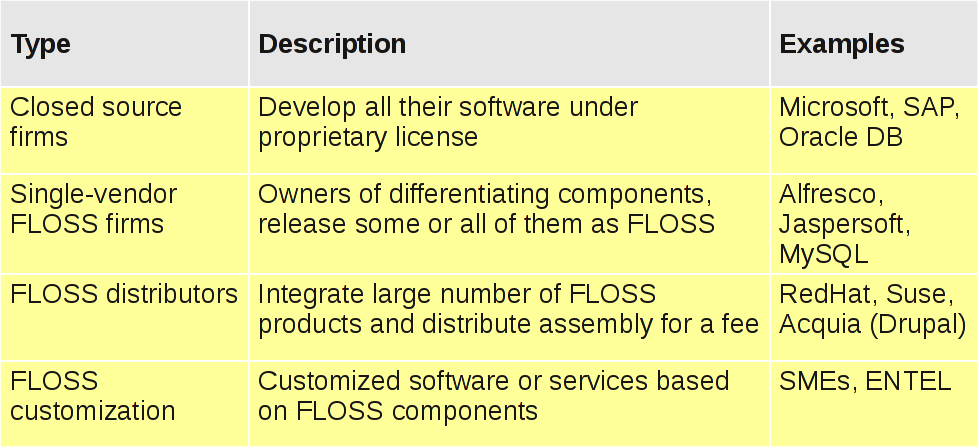
\includegraphics[width=10cm]{figs/sw-development-companies.png}
    \caption{Software companies according to business focus} 
  \end{figure}
\end{center}

\end{frame}

%%%%%%%%%%%%%%%%%%%%%%%%%%%%%%%%%%%%%%%%%%%%%%%%%%%%%%%%%%%%%%%%

\begin{frame}
 \frametitle{IPR strategies}
\begin{itemize}
 \item Two types of ownership strategies in FLOSS:
 \begin{itemize}
  \item \textit{Single-vendor FLOSS}: Only one legal owner of IPR, tipically a software development firm
that exerts itself to maintain its ownership rights.
  \item \textit{Community FLOSS}: This software has either a diffuse group of owners (all code contributors)
or it is owned by a foundation, acting on behalf or all its members
 \end{itemize}
\end{itemize}

\end{frame}

%%%%%%%%%%%%%%%%%%%%%%%%%%%%%%%%%%%%%%%%%%%%%%%%%%%%%%%%%%%%%%%%

\begin{frame}
 \frametitle{FLOSS license strategies}
\begin{itemize}
 \item Two types of strategies related to FLOSS licenses and business models:
 \begin{itemize}
  \item \textit{Reciprocal licenses (\textit{copyleft})}: Force any other company to release their own
products if they use, modify, distribute or integrate FLOSS components under the same license. 
Examples:GPL, AGPL.
  \item \textit{Permissive licences}: Do not force other companies to release their own product under a FLOSS
license if they use, modify, distribute or integrate FLOSS components. Examples: MPL, BSD.
 \end{itemize}
\end{itemize}

\end{frame}

%%%%%%%%%%%%%%%%%%%%%%%%%%%%%%%%%%%%%%%%%%%%%%%%%%%%%%%%%%%%%%%%

\begin{frame}
 \frametitle{Strategic goals}
\begin{itemize}
 \item \textbf{Reduction of development costs}.
 \begin{itemize}
  \item Reuse of available libraries, components, pieces of code, etc. reduce development costs.
 \end{itemize}

 \item \textbf{Maximization of customer exposure}.
  \begin{itemize}
   \item Active promotion of FLOSS project to sell superior product faster and at lower cost (single-vendor).
  \end{itemize}

 \item \textbf{Minimization of competition}.
  \begin{itemize}
   \item FLOSS ecosystems favor strong competition among providers and stakeholders.
   \item Single-vendors and software distributors adopt certain strategies to keep advantage over competitors.
  \end{itemize}

\end{itemize}
\end{frame}

%%%%%%%%%%%%%%%%%%%%%%%%%%%%%%%%%%%%%%%%%%%%%%%%%%%%%%%%%%%%%%%%

\begin{frame}
\frametitle{Control points \& steering mechanisms}

\begin{center}
  \begin{figure}
    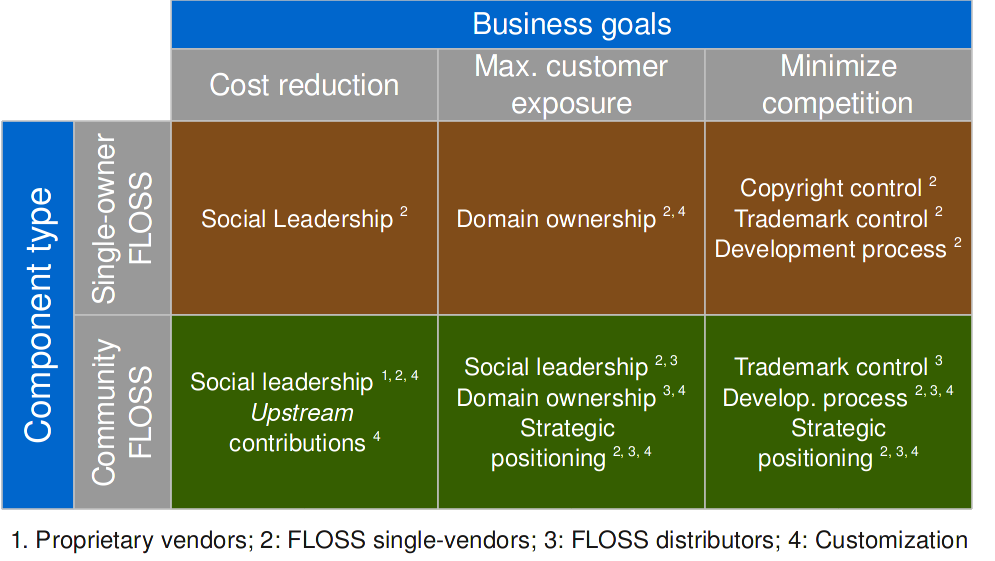
\includegraphics[width=10cm]{figs/control-steering-mechanisms.png}
    \caption{Control points and steering mechanisms in FLOSS business models} 
  \end{figure}
\end{center}

\end{frame}

%%%%%%%%%%%%%%%%%%%%%%%%%%%%%%%%%%%%%%%%%%%%%%%%%%%%%%%%%%%%%%%%

\begin{frame}
 \frametitle{Control points}
\begin{itemize}
 \item Can be enforced thanks to boundary conditions imposed by legal framework:
 \begin{itemize}
  \item \textit{Copyright control}: The company can grant certain rights through FLOSS licenses, but it also
can retain the exclusive copyright ownership. This prevents other third parties to release software under
a different license.
  \item \textit{Trademark control}: Trademarked names and logos deeply embedded in software. It will be costly 
(in terms of bot time and effort) to completely remove them to create \textit{clones}. As well, risk that 
original trademark owner can sue company removing trademarks, under the claim of unfair competition.
  \item \textit{Domain ownership}: Reinforced by trademarks, it contributes to show well-known corporate identity when customers
search for information.
 \end{itemize}
\end{itemize}

\end{frame}

%%%%%%%%%%%%%%%%%%%%%%%%%%%%%%%%%%%%%%%%%%%%%%%%%%%%%%%%%%%%%%%%

\begin{frame}
 \frametitle{Copyright practices}
\begin{itemize}
 \item Typically associated to single-vendor FLOSS firms.
 \begin{itemize}
  \item Requiring copyright transfer for any outside code contribution.
  \item Use reciprocal license to force competitors to release any differentiating improvement
under the same FLOSS lincense.
 \end{itemize}
  \item Copyright ownership enables multiple licensing.
  \item Growing use of licences like AGPL is expected as \textit{cloud} platforms become widespread.
\end{itemize}

\end{frame}

%%%%%%%%%%%%%%%%%%%%%%%%%%%%%%%%%%%%%%%%%%%%%%%%%%%%%%%%%%%%%%%%

\begin{frame}
 \frametitle{Trademark practices}
\begin{itemize}
 \item Important for distributors and single-vendor firms.
 \begin{itemize}
  \item Building a well-known, reliable corporate image to leverage associated products and services.
  \item Original owner will make it as hard as possible to remove any trademarks.
  \item No other competitor can benefit from original owner image.
  \item It fosters: partnerships, certification programs, etc.
 \end{itemize}

\end{itemize}

\end{frame}

%%%%%%%%%%%%%%%%%%%%%%%%%%%%%%%%%%%%%%%%%%%%%%%%%%%%%%%%%%%%%%%%

\begin{frame}
 \frametitle{Domain ownership practices}
\begin{itemize}
 \item Single-vendor firms and distributors use it to protect their own IPR.
 \item Customization companies use it to leverage their added-value and expertise in the market.
 \item Applied in combination with trademarks.
\end{itemize}

\end{frame}

%%%%%%%%%%%%%%%%%%%%%%%%%%%%%%%%%%%%%%%%%%%%%%%%%%%%%%%%%%%%%%%%

\begin{frame}
 \frametitle{Steering mechanisms}
\begin{itemize}
 \item \textit{Social leadership}: Community leadership may contribute
to participate in the definition of community culture, development practices,
evolution plan, partnerships, etc.
 \item \textit{Development process}: Hiring developers, private development process,
delayed distribution.
 \item \textit{Strategic positioning}: Benefit from foundation or alliance to
improve dissemination and public image, keeping advantage over competitors.
\end{itemize}

\end{frame}

%%%%%%%%%%%%%%%%%%%%%%%%%%%%%%%%%%%%%%%%%%%%%%%%%%%%%%%%%%%%%%%%

\begin{frame}
 \frametitle{Social leadership and upstream contributions}
\begin{itemize}
 \item Single-vendor firms employ featured developers, thus influencing the evolution of the FLOSS community
around that product.
 \item Proprietary vendors and customization firms support communities to reduce costs, reusing software components.
 \item Upstream contributions both improve leadership withing the community, and they guarantee compliance with the
source FLOSS components.
\end{itemize}

\end{frame}

%%%%%%%%%%%%%%%%%%%%%%%%%%%%%%%%%%%%%%%%%%%%%%%%%%%%%%%%%%%%%%%%

\begin{frame}
 \frametitle{Development practices}
\begin{itemize}
 \item The company can choose to follow private development process, so all improvements remain hidden from competitors.
 \item It can also decide to delay the release of improvements.
 \item Finally, competitor may only get snapshots of the code base, instead of the full revisioin history of the code repository.
 \item Hide future lines of work from competitors.
\end{itemize}

\end{frame}

%%%%%%%%%%%%%%%%%%%%%%%%%%%%%%%%%%%%%%%%%%%%%%%%%%%%%%%%%%%%%%%%

\begin{frame}
 \frametitle{Strategic positioning}
\begin{itemize}
 \item Usually associated to creation of FLOSS foundation, adding visibility, credibility and
optionally, neutrality.
 \item Example: ASF enforces diversity among developers of new accepted projects.
 \item Legal coverage for distributed copyright ownership.
 \item The foundation may act as a marketing channel to maximize customer exposure.
 \item Single-vendor firms can also leverage strategic baseline communities, to foster innovation in
``low risk'' products, then pick the best contributions to improve enterprise level products.
\end{itemize}

\end{frame}

%%%%%%%%%%%%%%%%%%%%%%%%%%%%%%%%%%%%%%%%%%%%%%%%%%%%%%%%%%%%%%%%

\begin{frame}
 \frametitle{Conclusions}
\begin{itemize}
 \item The business model is just the first step to define the global business strategy of companies.
 \item Around that business model, we need to select adequate control points and steering mechanisms
that will better contribute to ensure its sustainability.
 \item We cannot forget certain conditions:
  \begin{itemize}
   \item Get ready to rapidly react to changes in surrounding market conditions: competitors, partners,
clients, etc.
   \item Understand the advantages of new business relationships: \textit{co-opetition, commoditization, open innovation}, etc.
  \end{itemize}

\end{itemize}

\end{frame}

%%%%%%%%%%%%%%%%%%%%%%%%%%%%%%%%%%%%%%%%%%%%%%%%%%%%%%%%%%%%%%%%

\begin{frame}
 \frametitle{References}
\begin{itemize}
 \item Control points and steering mechanisms in open source software projects.
  \begin{itemize}
  \item \footnotesize{\texttt{http://dirkriehle.com/publications/2010/control-points-}}
    \footnotesize{\texttt{and-steering-mechanisms-in-open-source-software-projects/}}
  \end{itemize}
\end{itemize}

\end{frame}

%%%%%%%%%%%%%%%%%%%%%%%%%%%%%%%%%%%%%%%%%%%%%%%%%%%%%%%%%%%%%%%%